\section{Introduction}\label{sec:intro}

Hypergraph learning aggregates information through group relations
\cite{feng2019hgnn,chien2022allset}. When predictions determine which
candidate relations are retained, one node prediction can change several
incident hyperedges at once. An independent-edge model can match every
retention probability while missing this joint variation. Risk assessment
must therefore specify how the predictions generating an operator vary.

Degree normalization introduces a second distinction. Matching the mean
raw relation operator does not generally match the mean normalized
operator, and raw fluctuation amplification need not survive
normalization. A third distinction arises with trained predictors:
sampling nodes independently from their estimated class frequencies
preserves their marginals but removes dependence induced by a shared
training run. These distinctions concern the same question:
\emph{how does node-induced dependence change normalized spectral risk,
and which prediction law must calibration preserve?}

We answer this question by connecting normalized conditional influence,
law-specific calibration, and repeated-run diagnostics. Conditional
expectations decompose the normalized operator into orthogonal
single-node influences and a remainder. A three-operator comparison then
distinguishes static degree weighting from dynamic normalization.
Keeping this mechanism analysis separate from monitoring permits a
standard finite-sample rank threshold with a precise probability target.
Finally, complete training runs test whether fitted node marginals
provide an adequate replacement law.

The contribution is this connection and its measured limits in
prediction-constructed hypergraphs. The conditional-expectation
decomposition and rank rule are established tools. Their application
shows why matching edge marginals, retaining node-induced dependence,
and retaining an entire training-run law are different requirements.
Experiments on controlled families, Cora-CC, and DBLP-CA evaluate these
requirements separately. Raw-operator amplification, cancellation, and
tail-risk results supply the mechanism foundation in
Appendices~\ref{sec:raw-mechanism} and~\ref{sec:raw-validation}; the
main analysis asks what remains true after normalization and calibration.

Finally, we extend the complete-run calibration protocol to two visual
object hypergraphs, NTU2012 and ModelNet40. These experiments test the
cross-domain behavior of fitted node-product and independent-edge
calibration, and distinguish marginal rank validity from the
conditional variability of a threshold estimated from finitely many
complete runs.

\subsection{Related work}
Matrix concentration controls independent matrix sums
\cite{tropp2012user} and matrix functions of independent variables
\cite{paulin2016efronstein}. Other dependence assumptions include
strong negative dependence and Markovian summands
\cite{amparore2025dependent,geuchen2024matrix}. Independence of node
coordinates does not imply independence of their induced edge events.
Our raw-operator comparison uses the classical ANOVA decomposition
\cite{hoeffding1948class}, related to overlap calculations for motif
counts \cite{matias2006motifs}; its normalized version retains the
conditional-expectation identity while changing the influences.
Decoupling \cite{delapena1999decoupling}, latent-position spectral
inference \cite{athreya2018statistical}, and hypergraph spectral
similarity \cite{hayhoe24spectral} address related operator questions
under their respective probability models.

Rank calibration uses exchangeability to control a new observation
jointly with the random calibration sample. This differs from requiring
the conditional error probability of every realized calibration sample
to equal a target \cite{vovk2012conditional}. Conformal risk control
extends split-conformal reasoning to expected monotone losses
\cite{angelopoulos2024crc}. We use the simpler scalar upper-tail rank
rule and prove its scope explicitly. The inference target is an
operator-deviation alarm under the declared law. Task-level performance
is a separate empirical outcome.

Structural-noise analysis and hyperedge refinement connect graph
reliability to learning performance
\cite{dong23structural,huang26trustworthy}. Here the learning task
motivates the relation construction, and spectral deviation under a
stated law serves as an upstream structural diagnostic. Its task-level
consequences require separate evaluation.

\section{Operators, Centers, and Prediction Laws}\label{sec:norm-model}

Fix a candidate hypergraph $E$ on $n$ nodes, with $|e|\ge2$.
For a prediction vector $Y$, define
\begin{equation}\label{eq:norm-operator}
\begin{aligned}
H_e&=\mathbf1_e\mathbf1_e^\top/|e|,&
a_e(Y)&=\ind{Y_u\text{ agree over }u\in e},\\
B(a)&=\sum_e a_eH_e,& A(a)&=B(a)+\kappa I,\\
D(a)&=\operatorname{diag}(A(a)\mathbf1),&
S(a)&=D(a)^{-1/2}A(a)D(a)^{-1/2}.
\end{aligned}
\end{equation}
The experiments use $\kappa=1$ and unit edge weights. Degrees are
recomputed for every draw: $d_v(a)=\kappa+\sum_{e\ni v}a_e$.
Thus $S(a)\sqrt{d(a)}=\sqrt{d(a)}$ and $\|S(a)\|_2=1$.
This is the specified nonnegative symmetric operator; an implementation
using another HGNN normalization requires its own definition.

Under an independent categorical node law $P[u,c]$, model A draws the
entire $Y$ and constructs every $a_e(Y)$. Model B draws edge slots
independently with probabilities
$p_e=\sum_c\prod_{u\in e}P[u,c]$. Duplicate node sets share an event
in A but are independent slots in this counterfactual B model.
Both arms have $\mathbb E B=\sum_ep_eH_e$. For the fixed-degree control,
\begin{equation}\label{eq:fixed-degree}
D_0=\operatorname{diag}((\mathbb E B+\kappa I)\mathbf1),\qquad
S_0(a)=D_0^{-1/2}(B(a)+\kappa I)D_0^{-1/2},
\end{equation}
the means still match by linearity. Generally
$\mathbb E_A S\ne\mathbb E_B S$, and
$S(p)\ne\mathbb E_A S$. We report their roles separately.

\paragraph{Mechanism and monitoring centers.}
Mechanism comparisons use each arm's own mean in
$\|S-\mathbb E_{\mathrm{arm}}S\|_2$, with independently estimated
means in the simulations. Monitoring uses one center $\widehat M$
estimated in an independent reference stage and then frozen:
\begin{equation}\label{eq:monitor-score}
T(Y)=\|S(a(Y))-\widehat M\|_2.
\end{equation}
Comparisons between calibrators use the same center and scoring
pipeline. The deterministic baseline $S(p)$ is used only for local
response analysis, not as an interchangeable estimate of $\mathbb E S$.

\paragraph{Three prediction-law levels.}
L1 specifies a known product law for node predictions and tests its
induced joint relation law. The synthetic error profiles use benchmark
labels to define this model; they are not estimates obtainable without
labels at deployment. L2 estimates node class frequencies in an
independent reference stage and resamples from their product. Its
validity within that fitted law does not establish validity for the
actual training process. L3 treats an entire prediction vector from
one training run as one observation. Exchangeability is required across
runs of the same protocol, rather than across nodes. Random labeled
sets, random training partitions, and initialization with a fixed
training set define separate L3 mechanisms.

Figure~\ref{fig:calibration-map} separates two parts of the analysis.
The operator chain isolates static degree weighting from dynamic degree
recomputation, while each prediction law supplies complete relation draws
to the same normalized scoring pipeline.
\Needspace{12cm}
\begin{figure}[H]
\centering
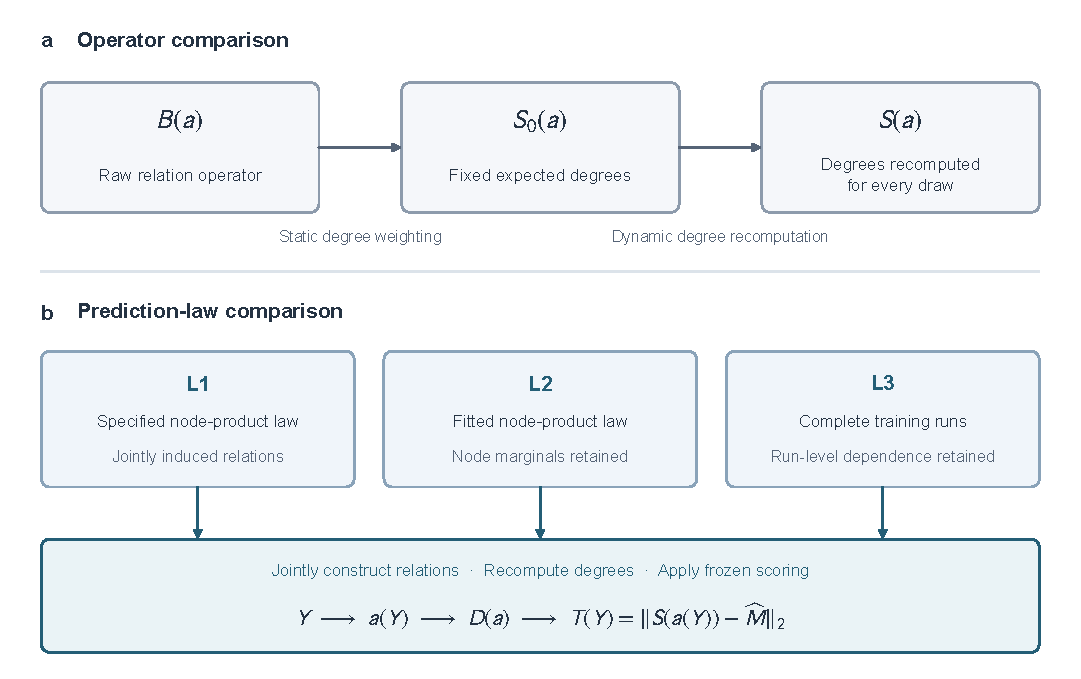
\includegraphics[width=\textwidth]{figures/operator_law_map.pdf}
\caption{The operator comparison and the prediction-law comparison are
distinct axes. (a) $B\to S_0\to S$ separates static weighting from dynamic
normalization. (b) L1--L3 specify which joint prediction mechanism generates
the relation draws used by the same normalized score.}
\label{fig:calibration-map}
\end{figure}

\section{Normalized Node Influence}\label{sec:normalized-influence}

Normalization changes the conditional response, but it does not remove
the conditional-expectation decomposition. Let
$X^S=S(Y)-\mathbb E S(Y)$ under L1 and define
\begin{equation}\label{eq:normalized-influence}
F_u^S(z)=\mathbb E[S(Y)\mid Y_u=z]-\mathbb E S(Y),\qquad
R^S=X^S-\sum_uF_u^S(Y_u).
\end{equation}

\begin{proposition}[Normalized conditional influence]\label{prop:norm-influence}
For independent node coordinates and finite second moments,
$\mathbb E[R^S\mid Y_u]=0$ for every $u$, and
\begin{equation}\label{eq:norm-energy}
\mathbb E\|X^S\|_F^2
=\sum_u\mathbb E\|F_u^S(Y_u)\|_F^2+\mathbb E\|R^S\|_F^2.
\end{equation}
For a binary coordinate with $P_0P_1>0$, put
$\Delta_u=\mathbb E[S\mid Y_u=1]-\mathbb E[S\mid Y_u=0]$.
Then $F_u^S(1)=P_0\Delta_u$, $F_u^S(0)=-P_1\Delta_u$, and
$v_u:=\mathbb E\|F_u^S(Y_u)\|_F^2=P_0P_1\|\Delta_u\|_F^2$.
\end{proposition}
\begin{proof}
Every $F_u^S$ has mean zero. For $v\ne u$, independence gives
$\mathbb E[F_v^S(Y_v)\mid Y_u]=0$, so conditioning
\eqref{eq:normalized-influence} on $Y_u$ gives zero conditional
remainder. Distinct influences, and each influence with the remainder,
are orthogonal in the expected Frobenius inner product. Expanding the
squared norm proves \eqref{eq:norm-energy}. The two binary values follow
by subtracting $P_0\mathbb E[S\mid0]+P_1\mathbb E[S\mid1]$.
\end{proof}

The proposition is the classical first-order decomposition applied to
the normalized matrix function. It identifies structure beyond degree:
two nodes with the same incident-edge count can have different
$\Delta_u$ because the remaining class profiles reinforce or cancel.
It does not assert that first-order influence dominates the remainder.
The raw-operator separation and cancellation theorems in
Appendix~\ref{sec:raw-mechanism} make their additional structure
conditions explicit. Their exact conclusions do not transfer
automatically through dynamic normalization.

The three-operator comparison makes that transfer measurable. Static
weighting changes $B$ into $S_0$, retaining common expectations. Dynamic
degrees change $S_0$ into $S$ and can change both means and fluctuations.
We therefore report a centered-norm ratio and a separate mean shift,
rather than interpreting a common-center difference as fluctuation
alone. Local derivative channels and a general perturbation bound are
given in Appendix~\ref{app:normalized-diagnostics} as supporting analysis.

\section{Calibration under a Stated Prediction Law}\label{sec:calibration}

\subsection{Reference, calibration, and evaluation}
The input is a fixed candidate hypergraph, its prediction-to-relation
map, a specified prediction law, and a target upper-tail probability
$\alpha$. The output is a frozen center, a threshold, and the law under
which the threshold is justified. The procedure has three stages.
\begin{enumerate}
\item Use independent reference observations to estimate $\widehat M$
and freeze all choices defining the score. For L2, estimate the product
law here; for L3, an observation is a complete training run.
\item Generate $M$ independent calibration observations from the chosen
law, construct all relations jointly, recompute degrees, and obtain
$T_1,\ldots,T_M$ with the frozen score.
\item For evaluation, keep the center and threshold fixed. Neither new
scores nor evaluation labels update the calibrator.
\end{enumerate}
The edge-independent baseline replaces step 2 by independent edge-slot
sampling at the same specified or fitted marginals. This changes the
calibration law; it does not inherit the node-law guarantee.

\subsection{Rank threshold and its probability target}
Let $T_{(1)}\le\cdots\le T_{(M)}$ and define
\begin{equation}\label{eq:rank-threshold}
k=\left\lceil(M+1)(1-\alpha)\right\rceil,\qquad
q_\alpha=\begin{cases}T_{(k)},& k\le M,\\+\infty,& k>M.\end{cases}
\end{equation}
An alarm is the strict event $T_{\mathrm{new}}>q_\alpha$.

\begin{proposition}[Law-specific rank validity]\label{prop:rank}
Condition on the independent reference stage. If the calibration
scores and a new score are exchangeable under a law $\mathcal L$, then
\begin{equation}\label{eq:rank-validity}
\Pr_{\mathcal L}\{T_{\mathrm{new}}>q_\alpha\mid\mathrm{reference}\}
\le\alpha.
\end{equation}
The probability averages jointly over calibration observations and
the new observation. With ties, the strict rule is conservative.
\end{proposition}
\begin{proof}
Break ties by independent random ordering. Exchangeability makes the
new observation's rank uniform on $1,\ldots,M+1$. Strict exceedance of
the $k$th calibration score implies a rank greater than $k$, giving
probability at most $(M+1-k)/(M+1)\le\alpha$. Removing the random
tie-breaking can only remove strict exceedances. If $k>M$ the event is
empty.
\end{proof}

This is the standard rank argument \cite{vovk2012conditional}.
Within L1 it applies to node draws and their jointly induced edges.
Within a frozen fitted product law it applies to L2 draws from that law,
not automatically to real training runs. Under L3 it applies to fresh
exchangeable complete runs of the same protocol. Repeatedly resampling
a finite run pool is not itself evidence of exchangeability with a
fresh training run.

\subsection{Interpreting empirical exceedance}
The realized threshold's conditional exceedance probability need not
equal $\alpha$ or satisfy \eqref{eq:rank-validity} conditional on that
particular calibration sample. Binomial Clopper--Pearson intervals
describe evaluation variability for a frozen threshold; including
$\alpha$ in such an interval does not prove equivalence. Across batches
with different fitted centers and thresholds, pooled evaluation
indicators need not have a common success probability. We report
batch-specific intervals or their explicitly labeled endpoint envelope.

\section{Experiments}\label{sec:exp}

The main experiments ask three consecutive questions: what
normalization changes, whether the chosen law supports calibration,
and whether a fitted node product reproduces complete training runs.
Cora-CC and DBLP-CA use AllSet benchmark inputs
\cite{chien2022allset}; their candidate structures contain 2,708/41,302
nodes and 1,579/22,363 edge slots. The controlled normalization families
use 120 edges per hub and are distinct from the larger raw-operator
grids retained in Appendix~\ref{sec:raw-validation}. All numerical
comparisons use the operator in \eqref{eq:norm-operator}.

\paragraph{Numerical and statistical protocol.}
Reference, calibration, and evaluation stages use separate seed streams.
Small matrices use dense symmetric eigendecomposition. Larger matrices
use both algebraic ends of a sparse eigensolver with a fixed start,
and the implementation can return an approximation or fallback score.
The rank guarantee applies to the shared implemented score, not to a
certified exact spectral norm. For large-scale DBLP matrices, raw and
fixed-degree spectral scores are computed with iterative sparse
eigensolvers as point estimates (marked with $\dagger$ in
Table~\ref{tab:normalization}), whereas rank-calibration guarantees
apply directly to the shared implemented scoring pipeline.

\subsection{Normalization changes the dependence comparison}
Dynamic normalization attenuated the estimated centered-norm ratio on
all displayed native units, while their computed ratios remained above
one (Table~\ref{tab:normalization}). The native dynamic ratios ranged
from 1.03 to 1.26, compared with raw ratios of 2.15--3.47.
The coherent controlled family instead changed from 2.93 for $B$ to
0.24 for $S$, accompanied by a normalized mean shift of 0.532.
These outcomes separate raw amplification from normalized behavior.
They do not attribute a fluctuation difference to mean shift alone,
because the ratios use each arm's own estimated mean.

% Generated from frozen results by notes/calibration-integration/generate_tables.py
\begin{table}[htbp]
\centering\small
\setlength{\tabcolsep}{4pt}
\begin{tabular}{llrrrr}
\toprule
Structure & Profile & $R_B$ & $R_{S_0}$ & $R_S$ & $\Delta_\mu$ \\
\midrule
Coherent & aligned & 2.93 & 1.16 & 0.24 & 0.53 \\
Competition & $\gamma=.05$ & 1.01 & 1.00 & 1.00 & 0.02 \\
Competition & $\gamma=.50$ & 1.40 & 1.02 & 0.99 & 0.09 \\
Competition & $\gamma=.95$ & 2.28 & 0.85 & 0.53 & 0.44 \\
Cora & binary .05 & 3.25 & 1.39 & 1.24 & 0.08 \\
Cora & binary .15 & 2.93 & 1.41 & 1.09 & 0.18 \\
Cora & multi .05 & 3.47 & 1.24 & 1.26 & 0.08 \\
Cora & multi .15 & 3.28 & 1.29 & 1.11 & 0.17 \\
Cora & hetero & 3.23 & 1.45 & 1.05 & 0.23 \\
DBLP$^\dagger$ & binary .05 & 2.48 & 1.70 & 1.13 & 0.19 \\
DBLP$^\dagger$ & binary .15 & 2.16 & 1.42 & 1.03 & 0.29 \\
DBLP$^\dagger$ & hetero & 2.15 & 1.77 & 1.07 & 0.34 \\
\bottomrule
\end{tabular}
\caption{Computed mean centered-norm ratios A/B; $\Delta_\mu=\|\widehat{\mathbb E}_A S-\widehat{\mathbb E}_B S\|_2$. Dynamic norms use each arm's own estimated mean; raw and fixed-degree means match analytically. Center/evaluation budgets per arm are 800/600 for the controlled families and Cora, and 120/80 for DBLP. Native binary/multiclass profiles have the displayed error probability; hetero uses binary errors at .02 below the upper degree decile and .30 within it. $\dagger$ DBLP raw/fixed-control scores include numerical approximations; these are point estimates, not certified norm ratios.}
\label{tab:normalization}
\end{table}


Exact small-graph enumeration verified the normalized conditional
orthogonality and energy identity to numerical precision. On the
degree-120 controlled hubs, estimated $v_u$ was 1.099 for the coherent
profile, approximately zero at the competing flat profile, and 1.311
at the aligned competing-family endpoint. Thus equal degree did not
fix normalized influence energy. Native influence estimates used
selected high-impact and background nodes; no full-native energy
closure is claimed.

\subsection{Model-law calibration and separate-seed reanalysis}
Preserving node-induced relations sharply changed calibration under
known node laws (Table~\ref{tab:node-calibration}). At target $\alpha=5\%$,
native node-calibrated batch means ranged from 3.9\% to 5.9\%, while
independent-edge thresholds yielded 47.5\%--100\% exceedance under the
same node mechanism. These are model-law comparisons: the labels used
to define the artificial errors are known to the simulator. Heterogeneous
calibration profiles use multiclass errors; the heterogeneous normalization
profiles in Table~\ref{tab:normalization} instead use binary errors.

% Generated from frozen results by notes/calibration-integration/generate_tables.py
\begin{table}[htbp]
\centering\small
\setlength{\tabcolsep}{4pt}
\begin{tabular}{llrr}
\toprule
Structure & Profile & Node (\%) & Edge-iid (\%) \\
\midrule
Cora & binary .05 & 5.2 [3.7,7.2] & 99.5 [98.3,100.0] \\
Cora & binary .15 & 5.0 [3.6,6.7] & 97.7 [95.6,99.4] \\
Cora & hetero & 5.9 [3.0,9.3] & 47.5 [40.5,54.9] \\
Cora & multi .05 & 4.8 [3.3,6.5] & 99.7 [98.7,100.0] \\
Cora & multi .15 & 5.5 [2.9,8.3] & 99.0 [97.5,99.9] \\
DBLP & binary .05 & 4.6 [1.4,9.3] & 100.0 [98.8,100.0] \\
DBLP & binary .15 & 5.1 [1.4,10.1] & 96.8 [90.7,99.8] \\
DBLP & hetero & 3.9 [0.9,8.9] & 99.7 [97.1,100.0] \\
Coherent & aligned & 0.0 [0.0,0.2] & 9.2 [7.8,10.7] \\
\bottomrule
\end{tabular}
\caption{Known-node-law exceedance at $\alpha=5\%$. Native entries are means over three independent threshold batches; brackets give the minimum lower and maximum upper endpoint of their individual 95\% binomial intervals, not a pooled 95\% interval. Per-batch reference/calibration/evaluation budgets are 200/500/1000 on Cora and 80/150/300 on DBLP. Hetero here uses multiclass errors at .02/.30. The coherent-family row is one batch with 400/800/1600 observations.}
\label{tab:node-calibration}
\end{table}


The controlled coherent family illustrates conservative ties. Its
5\% node threshold had zero strict exceedances in 1,600 evaluations,
because a discrete upper-tail atom determined the threshold. Zero
exceedance does not establish useful detection power, even when rank
validity holds. In the fitted-law Cora pilot, the three-repeat mean
5\% exceedance was approximately 5.0\% within the fitted model and
4.9\% under the specified generating law. That observation concerns
a weak-error synthetic product law, not the training-induced L3 law.

A fresh three-batch Cora rerun produced rates of 6.9\%, 3.3\%, and
4.9\%, for a mean of 5.03\% across 3,000 evaluations
(Table~\ref{tab:cora-rerun}). The batch-specific 95\% intervals have
an endpoint envelope of 2.28\%--8.65\%. Because centers and thresholds
differ by batch, this envelope is not a pooled interval. The three-batch
mean exceedance rate was 5.03\%, consistent with the nominal 5\% target
at this resolution.

% Generated from frozen results by notes/calibration-integration/generate_tables.py
\begin{table}[htbp]
\centering\small
\setlength{\tabcolsep}{4pt}
\begin{tabular}{rrrrr}
\toprule
Batch & Exceedances & Rate (\%) & CP 95\% interval & $q_{.05}$ \\
\midrule
1 & 69/1000 & 6.9 & [5.4,8.7] & 0.790 \\
2 & 33/1000 & 3.3 & [2.3,4.6] & 0.764 \\
3 & 49/1000 & 4.9 & [3.6,6.4] & 0.782 \\
\bottomrule
\end{tabular}
\caption{Fresh Cora-CC rerun under the specified binary node-product law. Each batch uses 200/500/1000 reference/calibration/evaluation draws and a distinct deterministic seed. Intervals are batch-specific conditional Clopper--Pearson intervals; the endpoint envelope is not a pooled interval. The three-batch mean exceedance rate was 5.03\%, consistent with the nominal 5\% target at this resolution.}
\label{tab:cora-rerun}
\end{table}


\subsection{Complete training runs expose product-law mismatch}
The product of empirical node frequencies produced zero observed
exceedances in every displayed L3 setting (Table~\ref{tab:run-calibration}).
Whole-run thresholds instead produced nonzero exceedances with broad
conditional intervals. In the two fixed-training-set GCN settings,
the run-pool counts at 5\% were 1/60 on Cora and 1/40 on DBLP;
the corresponding node-product counts were zero. These observations
support using complete runs as the practical calibration baseline for
the tested mechanisms. They do not establish uniqueness or universal
superiority of this baseline.

% Generated from frozen results by notes/calibration-integration/generate_tables.py
\begin{table}[htbp]
\centering\small
\setlength{\tabcolsep}{4pt}
\begin{tabular}{lllrrr}
\toprule
Data & Mechanism & R/C/E & Run-pool (\%) & Node-fit & Edge-iid \\
\midrule
Cora & LP & 50/100/100 & 4.0 [1.1,9.9] & 0.0 & 0.0 \\
DBLP & LP & 40/80/80 & 6.2 [2.1,14.0] & 0.0 & 0.0 \\
Cora & Proto & 30/100/150 & 3.3 [1.1,7.6] & 0.0 & 9.3 \\
DBLP & Proto & 20/50/80 & 6.2 [2.1,14.0] & 0.0 & 0.0 \\
Cora & GCN-XF & 20/40/60 & 6.7 [1.8,16.2] & 0.0 & 0.0 \\
Cora & GCN-init & 20/40/60 & 1.7 [0.0,8.9] & 0.0 & 0.0 \\
DBLP & GCN-init & 15/25/40 & 2.5 [0.1,13.2] & 0.0 & 0.0 \\
\bottomrule
\end{tabular}
\caption{Whole-run evaluation at $\alpha=5\%$. R/C/E are the reference/calibration/evaluation run counts. All rates are percentages; run-pool brackets are conditional 95\% binomial intervals for the realized threshold. LP varies labeled subsets, Proto varies a half split, GCN-XF uses five-fold cross-fitting, and GCN-init holds a 20\% labeled subset fixed. Zero node-fit counts do not imply zero population probability; their upper 95\% endpoints range from 2.4\% to 8.8\%. Every 5\% threshold displayed is finite.}
\label{tab:run-calibration}
\end{table}


The random mechanisms differ deliberately. LP varies the labeled
subset; prototype prediction varies a half split; cross-fit GCN varies
fold assignments and initialization. The final two rows hold a 20\%
labeled subset fixed and vary initialization only, using 500 epochs on
Cora and 120 on DBLP. The calibration/evaluation separation is at the
run level in each case. No DBLP cross-fit GCN row is inferred from the
fixed-split experiment.

At $\alpha=10\%$, the fixed-split run-pool counts were 9/60 on Cora
and 1/40 on DBLP. Their intervals included the target but were too
wide to establish equivalence. At $\alpha=1\%$, calibration pools of
25, 40, 50, or 80 runs cannot yield a finite threshold under
\eqref{eq:rank-threshold}; zero alarms at $q=\infty$ convey no
detection ability. More simulation from a fitted node product cannot
repair missing dependence in the model being simulated.

\subsection{Cross-domain calibration on visual object hypergraphs}\label{sec:visual}
We extended the complete-run protocol to two preprocessed visual object
hypergraphs from the ED-HNN benchmark~\cite{wang2023edhnn}: NTU2012 (2,012 objects, 67
classes, 2,012 five-object hyperedges) and ModelNet40 (12,311 objects,
40 classes, 12,311 five-object hyperedges). Object features and labels
were matched to the released incidence data by identifier, excluding
auxiliary hyperedge-node rows. A two-layer fixed propagation predictor
$S_{\mathrm{all}}\mathrm{ReLU}(S_{\mathrm{all}}XW_1)W_2$ used a fixed
stratified 60/20/20 training/validation/test split. Its output generated
the monitored operator $S(Y)$. Each dataset supplied one batch of 30
reference, 99 calibration and 200 independent evaluation runs, for
658 complete training runs across the two datasets.

The fitted node-product calibration remained conservative across
these visual domains (Table~\ref{tab:visual-alarm-validation}). At
$\alpha=5\%$, it yielded zero exceedances in 200 evaluation runs on
each dataset (upper CP endpoint $1.83\%$), extending the direction
observed on Cora-CC and DBLP-CA. Independent-edge calibration instead
yielded 10/200 exceedances on NTU and 53/200 ($26.5\%$) on ModelNet.
Thus preserving edge marginals or fitted node marginals did not
reproduce the calibration behavior of the complete-run law.

% Generated from frozen visual_alarm_v1 results by notes/calibration-integration/generate_tables.py
\begin{table}[t]
\centering\small
\setlength{\tabcolsep}{3pt}
\begin{tabular}{lccccc}
\toprule
Dataset & \multicolumn{3}{c}{Clean exceedance (\%; 95\% CP interval)} & Resplit & Time (s) \\
\cmidrule(lr){2-4}
 & L3 & L2 & Edge-iid & mean (\%) & train/score \\
\midrule
NTU2012 & 14.0 [9.5,19.6] & 0.0 [0.0,1.8] & 5.0 [2.4,9.0] & 5.0 & 3.5/0.04 \\
ModelNet40 & 5.5 [2.8,9.6] & 0.0 [0.0,1.8] & 26.5 [20.5,33.2] & 5.0 & 56.2/0.26 \\
\bottomrule
\end{tabular}
\caption{Cross-domain calibration at $\alpha=5\%$. Each dataset uses
30 reference, 99 calibration and 200 independent evaluation complete
runs. L3 calibrates on complete runs, L2 on a fitted node-product law,
and Edge-iid on independently sampled edge events. Brackets are
batch-specific $95\%$ Clopper--Pearson intervals. Resplit means use
10,000 random 99/200 partitions of the same 299 scores with a frozen
reference center; they are internal sensitivity summaries, not
independent validation. Timing gives median training/spectral-scoring
seconds per complete run under the recorded six-way parallel setup.}
\label{tab:visual-alarm-validation}
\end{table}


Complete-run calibration also exposes the distinction between marginal
and conditional validity. Its frozen threshold yielded 28/200
($14.0\%$) exceedances on NTU and 11/200 ($5.5\%$) on ModelNet.
Proposition~\ref{prop:rank} averages over the calibration
sample and the next exchangeable run; it does not require each frozen
threshold's conditional exceedance probability to equal $5\%$.
Figure~\ref{fig:visual-alarm-validation} compares the observed rates
with internal split sensitivity. With the reference center frozen,
10,000 random 99/200 splits of the same 299 NTU scores gave mean
exceedance $5.0\%$, median $4.5\%$, and 97.5th percentile $11.0\%$;
the original threshold lay at the 0.4th percentile of resampled
thresholds. ModelNet also gave a split mean of $5.0\%$. This
finite-pool rank check illustrates conditional variability; repeated
use of the same runs is not an independent population-level test of
the marginal guarantee.

\begin{figure}[t]
\centering
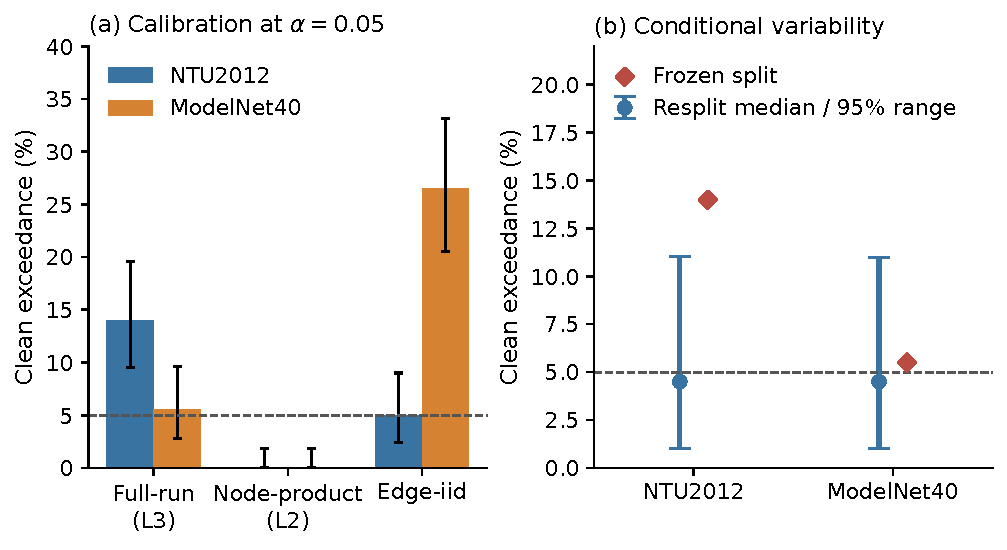
\includegraphics[width=\textwidth]{figures/visual_alarm_main.pdf}
\caption{Cross-domain calibration and frozen-threshold variability.
(a) Clean exceedance for complete-run (L3), fitted node-product (L2),
and independent-edge calibration at $\alpha=5\%$; horizontal error bars are
batch-specific $95\%$ Clopper--Pearson intervals from 200 evaluation
runs. (b) Original frozen-split rates and the median and central
$95\%$ range of 10,000 random 99/200 splits of the same 299 scores,
conditional on the frozen reference center. The split range is an
internal sensitivity summary, not a confidence interval for the
population risk. Dashed lines mark the $5\%$ target.}
\label{fig:visual-alarm-validation}
\end{figure}

A deployment requirement on the conditional risk of a frozen threshold
calls for an additional calibration criterion. Under an independently
and identically distributed run mechanism, a binomial tolerance rule
controls the probability that this conditional risk exceeds
$\alpha$, with confidence parameter $1-\delta$
\cite{vovk2012conditional}. At $M=99$ and
$\alpha=\delta=5\%$, it uses the 98th rather than the 95th ordered
score. On the same evaluation runs this gives 19/200 ($9.5\%$) on NTU
and 3/200 ($1.5\%$) on ModelNet. These realized rates remain distinct
from the rule's probability statement over calibration samples. The
tolerance comparison reuses the observed evaluation data; the
original thresholds and counts are retained. Appendix~\ref{app:visual}
gives the criterion, numerical sensitivity, and secondary
feature-perturbation comparisons.

\section{Discussion and Limitations}\label{sec:limits}

The results locate two distinct failures of a calibration shortcut.
Within a known independent-node model, treating induced edge events
as independent can produce severe over-exceedance. With real training
runs, a product of fitted node marginals can instead yield an overly
conservative threshold. The direction of failure depends on which
joint law is omitted. Consequently, preserving shared-node dependence
recovers the specified node-model construction but does not by itself
recover a training-run distribution.

Normalization explains why the raw theory is a starting point rather
than a sufficient calibration model. It can attenuate fluctuations,
shift expectations, or change the direction of a controlled comparison.
Conditional influence quantifies this change without assuming the
remainder is small. Its energy is structural information, not a proved
optimal monitoring direction. Appendix~\ref{app:normalized-diagnostics}
gives a local-response formula and perturbation bound as supporting tools.

The guarantees retain explicit boundaries. Known node laws need not
describe shared training states; fitted frequencies need not represent
repeated-run probabilities; and a fixed data set and training protocol
do not cover a new graph or a changed training process. The
Cora-CC/DBLP-CA L3 evaluation pools are small and lack a new
prospective confirmation with retained run-level prediction caches.
The visual protocol retains run-level caches for two additional
datasets under its stated single-batch 30/99/200 design. All runs in
a calibration claim must remain exchangeable under its declared
mechanism.

The visual benchmarks extend the distinction between joint laws to a
different data domain. Fitted node products remained conservative on
both, while independent-edge calibration gave substantial
exceedance on ModelNet40. The NTU frozen threshold and split-sensitivity
analysis further separate the probability target from any one
realization: marginal rank validity does not give a high-confidence
bound on the conditional risk of every deployed threshold. Binomial
tolerance calibration provides an established way to express the
latter objective under an independent-run model. More calibration
runs can reduce sampling variation, but the probability target and
assumed law must first be specified.

Numerical precision is a separate restriction. The DBLP entries in
Table~\ref{tab:normalization} are computed-score evidence; certified
spectral-norm magnitudes require an independent numerical audit. The ES
importance estimates also do not provide a usable tail certificate:
their effective-sample diagnostics were low and tested bounds were
vacuous. Stronger remainder bounds and risk-weighted propagation are
outside the present claim.

\section{Conclusion}\label{sec:conclusion}
Normalized spectral-risk calibration requires a declared joint
prediction law. Conditional influence separates the effects of
normalization from raw-operator fluctuation, while rank calibration
states validity under the corresponding exchangeability assumption.
Controlled families, citation networks and visual object hypergraphs
show different calibration consequences of omitting shared-node
relations or training-run dependence. Complete-run and split-sensitivity
comparisons further distinguish marginal validity from the conditional
behavior of a frozen threshold. These results guide the construction
and interpretation of upstream operator-deviation alarms.
